% for PsychSci APA6 TeXLive 2020 use this with biber/biblatex + styel=apa6
% figure note is not supported, put it in the caption
\documentclass[helv,10pt,man,floatsintext]{apa6}  %% man <-> jou <-> doc
\usepackage{csquotes}
\usepackage[backend=biber,style=apa6]{biblatex}
\addbibresource{apa_ms.bib}

% if you like line numbers ...
\usepackage{lineno}
%\linenumbers

\usepackage[american]{babel}
% \usepackage[utf8x]{inputenc}
\usepackage[utf8]{inputenc}
\usepackage{amsmath}
\usepackage{graphicx}
\usepackage{multirow}
\usepackage{multicol}
\usepackage{xcolor}


% for tracking changes
\usepackage[draft]{changes}
\definecolor{skyblue2}{rgb}{.203, .395, .640}
\definecolor{orange2}{rgb}{.957, .473, .000}
\definecolor{plum2}{rgb}{.457, .313, .480}
\definechangesauthor[name=TPU, color=skyblue2]{TPU}
\definechangesauthor[name=ABC, color=orange2]{ABC}
\definechangesauthor[name=XYZ, color=plum2]{XYZ}


% to include one or more pages of multipage pdfs
\usepackage{pdfpages}

% for cross-references back to the main doc
% use \zref{} and \zlabel{} instead of latex native \ref{} and \label{}
\usepackage[xr, user, titleref]{zref}
\zexternaldocument{apa_si}  % other .tex file to cross reference

% to help control location of figures and tables
% \usepackage{float}

% highlight computer source code
\definecolor{bgc}{rgb}{.96,.96,.96}
\usepackage{minted}
\setminted[latex]{
  xleftmargin=0.5in,
  xrightmargin=0.5in,
  style=bw,
  frame=none, % lines,
  bgcolor=bgc,
  fontsize=\footnotesize,
  linenos
}

% for clickable URL links in pdfs
\usepackage{hyperref}
\hypersetup{
    colorlinks=true,
    citecolor=blue,
    linkcolor=blue,
    filecolor=blue,      
    urlcolor=blue,
}

% use this to prevent LaTeX errors when urls break across pages
%% \hypersetup{draft}

\title{Open science data analysis with style: A reproducible repoducible research report}
  
\shorttitle{Analyzing data in style}

\author{Thomas P. Urbach}
\leftheader{Urbach}

\affiliation{
  Cognitive Science Department \\
  University of California, San Diego \\
  \today
}

\abstract{When the culmination of research is a research report, the
  culmination of reproducible research must be a reproducible
  report. To accomplish this, three problems must be solved: 1) the
  results of the reproducible data analysis must be incorporated into
  the narrative text, tables, and figures of the document; 2) the
  document must comply with the byzantine typographical requirements
  of professional publication style guides and their idiosyncratic
  modifications by various publishers; 3) the different parts and
  pieces of the report (manuscript, supplementary information,
  figures, tables, captions) must be reproducible digital objects in
  whatever specific document and image file format is required by the
  online platforms for submission to the journal and production by the
  publisher.  This report describes and demonstrates a flexible and
  generalizable approach that combines freely available open source
  data analysis and document preparation software tools to solve these
  three problems. The report itself is reproducibly generated by the
  approach it describes and demonstrates for psychologists with
  real-world examples: the manuscript is formatted in American
  Psychological Association style and the digital objects are
  generated as required for the online submission and production
  platforms used by {\it Proceedings of the National Academy of
    Sciences}. The source code is publicly available and may be cloned
  from the GitHub repository or downloaded from the Open Science
  Foundation archive and freely modified or adapted for non-commercial
  purposes under the Creative Commons
  Attribution-NonCommercial-ShareAlike 4.0 International (CC BY-NC-SA
  4.0) license. This reproducible report, together with the source
  code that reproduced it, comprise a complete self-contained
  tutorial, demonstration, and template for general use.  }

\begin{document}
\maketitle

\section{Introduction}

For any research project, after all the work of experimental design,
implementation, and data acquisition are in place, and the data
analysis is complete, there still remains the task of preparing and
publishing the peer-reviewed research report with a clear and accurate
presentation of the results through the text, tables, and
figures. However, the ``research report'' is an abstraction; in
practice it takes various forms on its trajectory from the authors'
desks to dissemination as a journal article in print and online in
digital form(s). For the authors, there all the usual chores of
document preparation: Writing the narrative text with qualitative and
quantitative analysis results, creating high-resolution graphics for
figures, preparing tables of data and results, adding and deleting
citations and bibliographic references, embedding links to URLs, and
aligning cross-references to elements within or across documents,
e.g., to the separate online supplementary information. During
preparation and revision the report is in flux and must be editable
with changes to the text tracked across versions.  For pre-print
archives and (re-)submission to peer-reviewed journals the text and
graphics are composited into a usually un-editable but easily
transmissible and viewable digital snapshot, e.g., typically Portable
Document Format (PDF). Finally, for journal and book publishers, the
process is unwound and the report must be comprised of separate
editable text and ``camera ready'' high-resolution graphics suitable
for production in digital form for online viewing and print
form. Throughout these transformations for publication, the report
must also satisfy specific style requirements and for psychologists
this often means a variation of the 6\textsuperscript{th} Edition of
the Publication Manual of the American Psychological
Association~(\cite{APAStyle6th}). Or maybe the 7th Edition. In short,
as a research report evolves from inception to DOI, it must sometimes
change and other times freeze in various highly specific forms and
digital file formats as it passes through different hands with
different requirements.

When the goal of reproducible research is fully embraced, the
``research report'' must also be reproducible throughout these stages
of preparation, revision, submission, and production. This requires
solving three problems: 1) the results of the reproducible data
analysis must be incorporated into the narrative text, tables, and
figures of the document; 2) the document must comply with the
byzantine typographical requirements of professional publication style
guides and their idiosyncratic modifications by various publishers; 3)
the different parts and pieces of the report (manuscript,
supplementary information, figures, tables, captions) must be
reproducible digital objects in whatever specific document and image
file format is required by the vagaries of an online journal
submission platform and then subsequently by a different online
production platform. Solutions to each of these problems individually
abound, the challenge is to combine them reproducibly. For instance,
reproducible data analyses are becoming commonplace though the use of
scientific computing platforms and open source scripting languages
like Python and R encapsulated in virtual environments (conda,
virtualenv) and containers (Docker, singularity). However the
technology for solving the data analysis problem is decoupled from the
strict typesetting requirements of different publication styles. On
the other hand, mature document preparation software like Microsoft
Word and \LaTeX{} provide the fine-grained control of formatting
necessary to comply with idiosyncratic style guidelines. However,
typing or copy-pasting the results decouples the report from the
analysis.  The results of the analysis may be reproducible when the
analysis is revised by co-authors or reviewers, but the results do not
propagate to all the digital objects that comprise the parts and
pieces of the report for (re-)submission and production.

This self-reproducing tutorial describes and demonstrates one approach
to solving all three problems at once using mature freely available
open-source computer software, a working knowledge of
\LaTeX{}~(\cite{latexproject}), and no more knowledge of computer
programming than is already required to implement the reproducible
data analysis it reports. The tutorial includes a sample reproducible
data analysis pipeline with open-access data but focuses mainly on the
reproducible report per se, i.e., solutions to the second and third
problem needed to bridge the gap between the end of the reproducible
data analysis and the DOI of the peer-reviewed publication in an
academic journal. In addition to programmatically combining the data
analysis results with the narrative text, tables, and figures of the
report, the complete \LaTeX{} source code listings in the
Supplementary Materials provide working examples of some features
generally useful for manuscript preparation: tracking changes across
revisions, preparing camera ready graphics, automating
cross-references within and between documents, formatting and masking
the citations and bibliography, generating Portable Document Files,
compositing documents and pieces of documents in text and PDF file
formats, and preparing an author's manuscript for distribution while a
published article is embargoed.  The Supplementary Information
provides instructions for installing the open source software required
to reproduce the data analysis and this report. The complete source
code for the data analysis and report generation is publicly available
and may be downloaded from the Open Science Foundation archive or
cloned from the GitHub repository under a Creative Commons CC BY 4.0
license~\cite{ccby4.0} and used as a template and freely modified for
other purposes with appropriate attribution.

\section{Method}

\begin{figure}[ht]
\caption{Generating a reproducible APA 6th style research report: 1)
  Executing the reproducible data analysis code generates the complete
  results which appear as-is in the Supplementary
  Information. Selected results to be reported in the manuscript are
  exported to separate files as minimally styled narrative text and
  tables, and PDF graphics. 2. The graphics exported by the analysis
  are converted to camera ready APA-style figure graphic PDFs for the
  manuscript. 3. The Supporting information \LaTeX{} file is typeset
  as a document PDF which includes the complete analysis source,
  results, graphics, and document source. 4. The \LaTeX{} manuscript
  is typeset as a document PDF which includes the results text
  generated by the data analysis, the camera ready PDF figures, and
  bibliography.}  \zlabel{ms:report_generation}
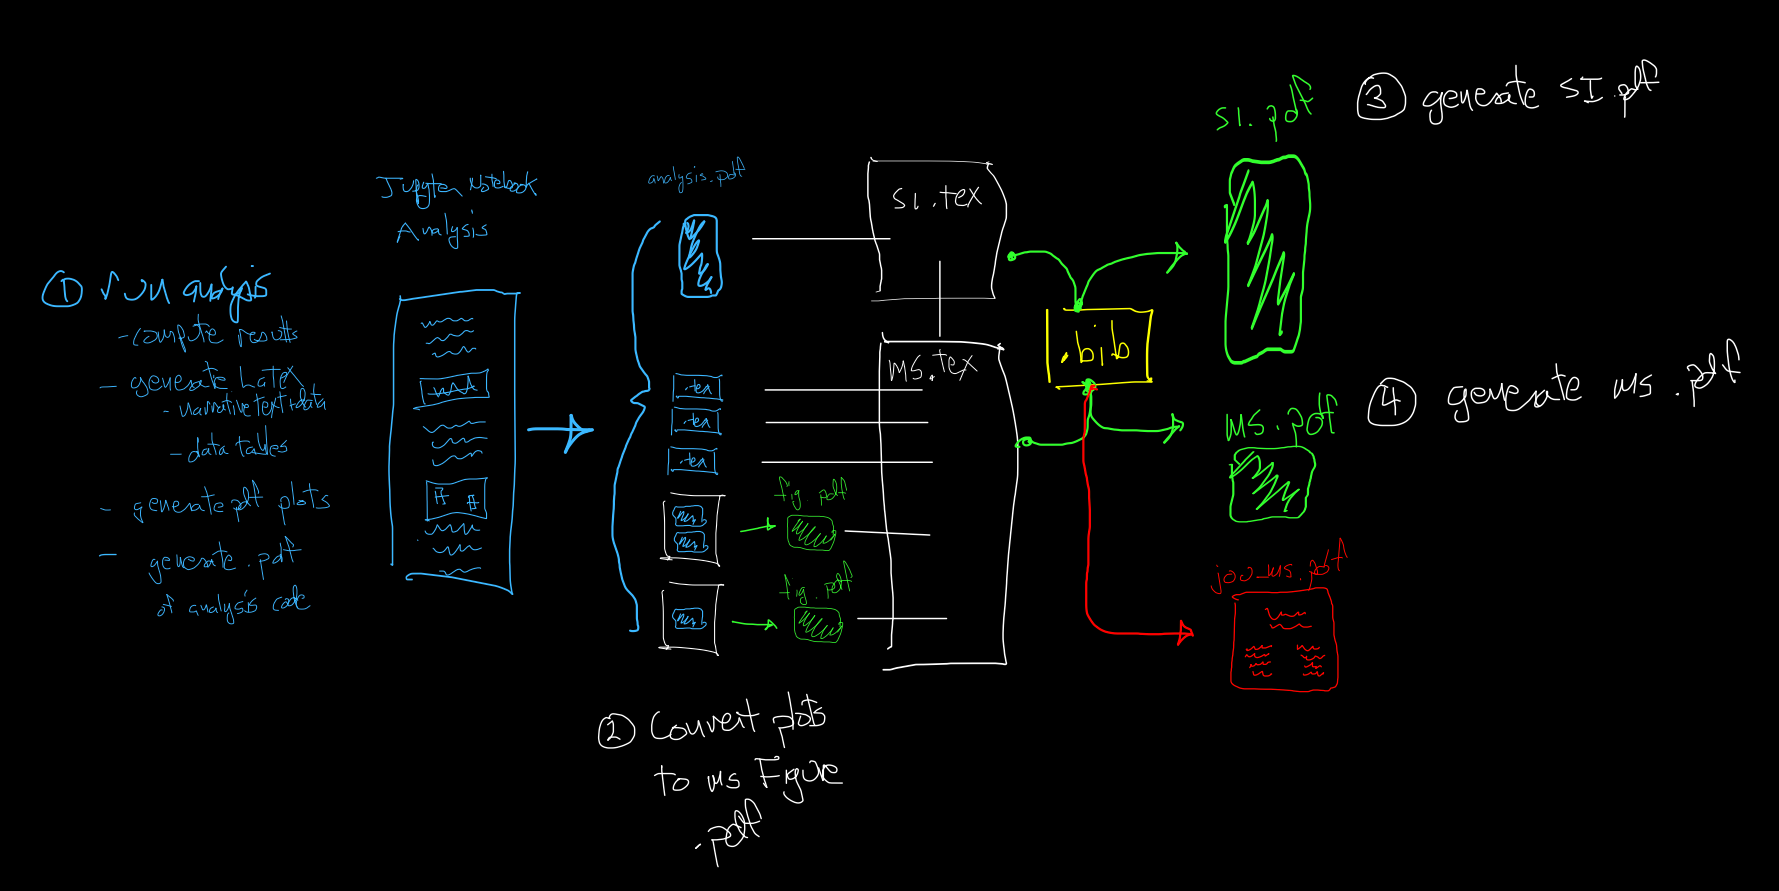
\includegraphics[width=.95\textwidth]{images/report_generation.png}

\end{figure}


This approach to generating reproducible research reports requires
the four main components, outlined schematically in
Figure~\zref{ms:report_generation}. While the approach is flexible and
generalizable, the specific examples are selected for researchers in
Psychology and demonstrate how to satisfy all the requirements (except
word count) for submitting and publishing a research report in the
journal, {\it Psychological Science}. Accordingly the manuscript is
structured with a Cover Page, Abstract, Introduction, Method, Results,
and Discussion~\parencite{APSStructStyle} and formatted according to
the APA 6th edition style~\parencite{APAStyle6th}. The approach here
is readily adapted to the APA 7\textsuperscript{th} Edition with a
change of the document
class~({\href{https://www.overleaf.com/project/5f3053af0af0dc00016f191b}{apa7}})
and minor modifications to the text described in Supporting
Information. The approach generalizes to other publication styles for
which \LaTeX{} style files have been defined.  A conveniently inventory
is collected here:
\href{https://www.overleaf.com/latex/templates/tagged/academic-journal}{Overleaf.com
  Templates\textemdash Academic Journal}. Many styles are community
contributions, for instance,
\href{https://www.overleaf.com/latex/templates/tagged/arxiv}{arXiv,
  bioRxiv}.
%
A number of journals and publishers provide official styles, such as
%
\href{https://www.overleaf.com/latex/templates/tagged/npg}{Nature},
\href{https://www.overleaf.com/latex/templates/tagged/pnas}{Proceedings of the National Academy of Sciences},
\href{https://www.overleaf.com/latex/templates/tagged/elife-official}{eLife}
%
and publishers
%
\href{https://www.overleaf.com/latex/templates/tagged/cup-official}{Cambridge University Press},
\href{https://www.overleaf.com/latex/templates/oup-general-template/fqkhysbcbpwv}{Oxford University Press},
\href{https://www.overleaf.com/latex/templates/tagged/springer}{Springer}
%
including 
%
\href{
  https://www.overleaf.com/latex/templates/a-demonstration-of-the-latex2e-class-file-for-sage-publications/jcdyknyjrkzb
}{
  SAGE
},
%
the publisher of {\em Psychological Science}.
%
The Supporting Information for this report provides installation
instructions for the necessary software and complete source code
listings for the analyses, documents, and figures which are freely
available under the CC-BY-4.0 license and may serve as templates for
a range of research projects in the psychological sciences.


\subsection{Data analysis pipeline: \mintinline{bash}{apa_analysis.ipynb}}

For demonstration purposes, a toy reproducible data analysis pipeline
is implemented in a Jupyter notebook running a Python
kernel~(\cite{kluEtAl2016}).  The pipeline (down)loads and
transforms a sample EEG dataset~(\cite{Urbach2020z}), computes summary
measures, and generates figures and text output. The particulars are
incidental, the data may as well be response times and the analysis
could be implemented in R, MATLAB, or any language that can format
numerical values as strings, write string variables to a text file,
and export as PDF, EPS, PNG, JPEG (or a format programmatically
convertible to one of these). This PDF is used for vector graphics and
PNG for raster graphics in this report since these have proved
reliable and both support transparency; EPS and JPEG also work if
these are required by the publisher.


\subsection{Preparing camera ready figures with \LaTeX{} and Ti{\it k}Z}

Ideally, graphic images generated by an analysis pipeline will be in
final ``camera ready'' form but this is not always practical or
possible.  A figure may require annotations, e.g., math notation, not
supported by the figure generator and a multipanel figure may need to
combine images from different sources. To demonstrate how this may be
done programmatically for reproducibility, three of the ``rough'' plot
graphics generated by the analysis pipeline are reconfigured, annotated
and converted into two camera-ready APA-style manuscript figures
(Figure~\zref{ms:multipanel} and Figure~\zref{ms:tikzfig}) using \LaTeX{} and
the Ti{\it k}Z graphic library without additional software or manual
editing.


\subsection{Manuscript: \mintinline{bash}{apa_ms.tex}}

LaTeX{} is a form of markup language where
the document text is intermingled with short typesetting
instructions. For instance, {\it this phrase is typeset in italics},
and the instruction looks like this:
%
\mintinline{latex}{{\it this phrase is typeset in italics}}.
%
Mathematical symbols and more complex equations are very
well-supported and set in the same way, e.g., partial eta squared
($\eta_p^2$) is set like so: \mintinline{latex}{$\eta_p^2$}.  Other
instructions are more general. For instance, the manuscript document
begins with this,
\mintinline{latex}{\documentclass[man,helv,10pt,draftall,floatsintext]{apa6}},
that says to typeset the document as a manuscript, in Helvetica 10
point font with a draft watermark on all pages, formatted to the APA
6th Edition style except that tables and figures should be placed near
where they appear in the text (``floatsintext'') rather than collected
at the end. This style, including the deviation from the APA 6th table
and figure position, corresponds to the submission guidelines for
Psychological Science~\parencite{PsychSciSubmissions2020}.  Like all
\LaTeX{} files, the main manuscript file is a plain text document and
thus virus-free, portable, viewable, and editable with any text
editor, although one that supports LaTeX syntax highlighting
on-the-fly syntax error checking is strongly recommended.

\subsubsection{Supplementary Information: \mintinline{bash}{apa_si.tex}}

Supplementary Information is as much a part of the report as the
manuscript and must be likewise reproducible. For demonstration here,
the Supplementary Information is comprised of a separate \LaTeX{}
file.  It provides instructions for downloading this report from
public repositories and installing the software to reproduce it. It
also includes source code listings of the Makefile used to reproduce
portions or all of the analysis, source code and output of the entire
executed analysis Jupyter notebook and listings of all the \LaTeX{}
files used to generate the report, figures, and supporting
information, which includes the self-reflexive listing of the
Supporting Information listing itself.


\subsection{Reproducing the report: \mintinline{bash}{Makefile}}

The \mintinline{bash}{make} program is a widely used command line
utility for managing the execution of a interdependent computer code
in complex programming projects, where changes in one file may might
impact some but not all other files. Reproducible data analysis and
report generation is similar in that, e.g., generating the
camera-ready figure PDFs depends on the rough plots generated by the
analysis which in turn depends on executing the analysis. The make
utility provides a useful mechanism for expressing the
interdependencies and comparmentalizing the project as work
progresses, e.g., \mintinline{bash}{make analysis} or
\mintinline{bash}{make fig2} or \mintinline{bash}{make ms} while
\mintinline{bash}{make all} ensures that all the components execute in
the correct order to completely reproduce the analysis and generate
all the files and documents for the figures, manuscript, supporting
information. Here is a summary of the make file components for
generating this report, execution times are for a high performance
workstation.

\begin{description}

\item [\mintinline{bash}{make analysis} (45 s)] Reproduce the data analysis by
  executing all the computer code in the analysis notebook start to
  finish. This has four side effects:

\begin{enumerate}
  \item The data analysis computations are executed and the results captured
    as standard output and plots in the Jupyter notebook cells. 
  \item Results to be included in the manuscript as narrative text and
    tables are embedded in text strings, minimally formatted to APA
    style with \LaTeX{}, and exported as separate text files (.tex).
  \item Plots to be included in the manuscript figures are exported as
    PDF graphics.
  \item After execution is complete, a snapshot of the complete
    notebook\textemdash text, computer code, and results captured in
    the output cells\textemdash is exported to a PDF file. The PDF is
    included in its entirety in the Supplementary Information.
\end{enumerate}  

\item [\mintinline{bash}{make fig1} (1 s)] Run
  \mintinline{latex}{pdflatex fig1.tex} to convert two rough plot
  graphics as generated by the analysis pipeline into the camera-ready
  Figure~\zref{ms:multipanel} graphic shown in the manuscript.

\item [\mintinline{bash}{make fig2} (1 s)] Run \mintinline{latex}{pdflatex fig2.tex}
  to convert the rough plot graphic generated by the analysis
  pipeline into the camera-ready Figure~\zref{ms:tikzfig} graphic shown in the
  manuscript.

\item [\mintinline{bash}{make figs} (47 s)] Execute the analysis to generate the rough PDF graphic
  output files then make fig1 and fig2 as above. 

\item [\mintinline{bash}{make ms} (9 s)] Run \mintinline{bash}{pdflatex apa_ms.tex}
  to generate the manuscript PDF.

\item [\mintinline{bash}{make si} (4 s)] Run \mintinline{bash}{pdflatex apa_si.tex}
   to generate the Supporting Information PDF.

\item [\mintinline{bash}{make all}] Run make figs to execute the
  analysis and generated camera ready figures then make ms and si
  enough times to update and the cross-references between the
  manuscript and supplementary information.

\end{description}


\label{sec:results}

\section{Results}

The results are this report and the Supplementary Information. Both
are reproducibly reproduced using freely available open source
software, a working knowledge of \LaTeX{} and no more computer
programming than the Python used for the data analysis.  A few points
merit further discussion.

\section{Discussion}

\subsection{Linking data and arbitrary text}

% This is the complete latex for this entire section
\input{generated/arbitrary_text.tex}


The listing below shows the minimally styled \LaTeX{} text generated
by the analysis pipeline. For illustration, it includes comments
(\%\%), narrative text with the data values filled in progrmmatically,
and \mintinline{latex}{{\it N }}, which italicizes the capital N
according to APA 6th style:

% this shows it as a source listting
\inputminted{latex}{generated/arbitrary_text.tex}


\subsection{Tables}

The ability to link data with arbitrary text is nowhere more valuable
than in preparing reproducible data tables styled to editorial
standards.  The primary challenges are the intricate requirements for
laying out headings and notes as illustrated by the following exerpts,
drawn from the 40 pages of APA Publication Manual 7th edition table
guidelines:

\begin{quote}
{\bf headings} Tables may include a variety of headings depending on
the nature and arrangement of the data. All tables should include
column headings, including a stub heading (heading for the leftmost
column). Some tables also include column spanners, decked heads, and
table spanners (see Section 7.12) 

\ldots

{\bf notes:} Thee types of notes (general, specific, and probabiity)
appear below the table as needed to describe contents of the table
that cannot be understood from the table title or body alone \ldots
\end{quote}

\noindent
It is straightforward to reproducibly link table text to the analysis
data they tabulate. It is less straightforward, but still tractable to
do while also generating the three types of notes, four types of
headings and column spanners, and ``a border at the top and bottom of
the table, beneath column headings (including decked heads), and above
column spanners.''  (p. 205)

The tabular exhibit labeled Table~\zref{ms:table1} illustrates a
not-quite conforming tabular array of data. When the analysis runs,
the table is reproducibly generated as a \LaTeX{} .tex file with one
line of code \mintinline{python}{pandas.DataFrame.to_latex()}. 
\footnote{
  For analyses scripted in R, the \mintinline{R}{xtable} library
  similarly generates \LaTeX{} format table from dataframes
  \url{https://cran.r-project.org/web/packages/xtable/index.html}.
}
The .tex file is imported into the manuscript the same way as the arbitrary
text file above.

\begin{table}[ht]
  \centering
  \caption{A non-APA Style data table and note generated
    as \LaTeX{} by calling \mintinline{python}{pandas.DataFrame.to_latex()}.} \zlabel{ms:table1}
  \begin{threeparttable}
    \input{generated/p3_table1.tex}
    \begin{tablenotes}[flushleft]
      Note: Python variables are conventionally lower case.
    \end{tablenotes}
  \end{threeparttable}
\end{table}

\noindent
This approach is simple and easy and well-suited for data tables
presented in supporting information where styling requirements are
typically less strict. When easily generated tables will not do, the
fall back is arbitrary text generation.  A few lines of Python code
and common string formatting methods suffice to generate the \LaTeX{}
required to format the table header, footer, notes and row data to APA
style. The following listing shows the programmatically generated
\LaTeX{}, the result is shown as Table~\zref{ms:table2}. The Python
source code to is Jupyter notebook in the~Supporting
Information.

\inputminted{latex}{generated/p3_table2.tex}


\begin{table}[ht]
  \centering
  \caption{An APA style data table and note generated as \LaTeX{} with
    a few lines of pure Python.}
  \zlabel{ms:table2}

  \centering
  \begin{threeparttable}
    \input{generated/p3_table2.tex}
    \begin{tablenotes}[para, flushleft]
      Note: APA Style capitalization.
    \end{tablenotes}
  \end{threeparttable}
\end{table}



\subsection{Figures}

Graphics figures in PNG, PDF, and JPEG can be included in a \LaTeX{}
document with the \mintinline{latex}{command}. Of these PDF seems to
be the most reliable for vector graphics (plots, line drawings,
charts, plots) and PNG for raster graphics.  Including figures is
straightforward, creating figures for a data analysis reproducibly is
another matter. In some case it may be possible to generate
camera-ready graphics from the data anlysis pipeline itself. Although
this takes some effort to fine tune at the outset when Reviewer 2
insists on some mid-stream revision that requires re-running the
analysis, the change propagates all the way through to the final
figures included in the report. However this is not always
possible. One recourse is to use an interactive vector graphics
manipulation programs like Inkscape to import the graphic and edit to
style but, like manually typing results into a data table, the results
may change but the representation of the results does not.

Since hand editing figures amounts to using a mouse to select a
sequence of drawing commands, it can be done programmatically with the
right vector graphics manipulation tools. In the LaTeX{} ecosystem, a
particularly powerful package for this is
\href{https://en.wikipedia.org/wiki/PGF/TikZ}{Ti{\it k}Z} and the
learning curve is correspondingly steep. However, for simple tasks
like laying out and annotating the figures, it is reasonably
straightforward. The tikz figure is a canvas with coordinates.
Graphics can be placed and aligned, and drawing elements like lines,
arrows, and shading added. Figure~\zref{ms:multipanel} and
Figure~\zref{ms:tikzfig} are worked examples of this approach and show
how to convert graphics generated by the data analysis into ``camera
ready'' figures to APAstyle specifications saved as separate PDF files
for upload to the publisher.  Figure~\zref{ms:multipanel} is a simple
example that lays out two graphics side by side and
Figure~\zref{ms:tikzfig} illustrates a more elaborate example that
selects portions of a single graphic, rearranges and resizes them and
adds additional graphic and text annotations. The \LaTeX{} and Ti{\it
  k}Z code for both figures is listed in the Supplemental Information.

\begin{figure}[ht]
  \caption{
    A complete multi-panel color figure generated
    reproducibly from the data to Psychological Science figure
    specifications. The figure is generated using the matplotlib package in
    Jupyter Notebook running a Python kernel. The code illustrates
    some useful Python idioms and matplotlib functionality including
    style sheets, the style context manager, how to lay out panels,
    add labels including with mathematical symbols, and export the figure as
     as a PDF graphic.
  }

  \zlabel{ms:multipanel}
  \centering
  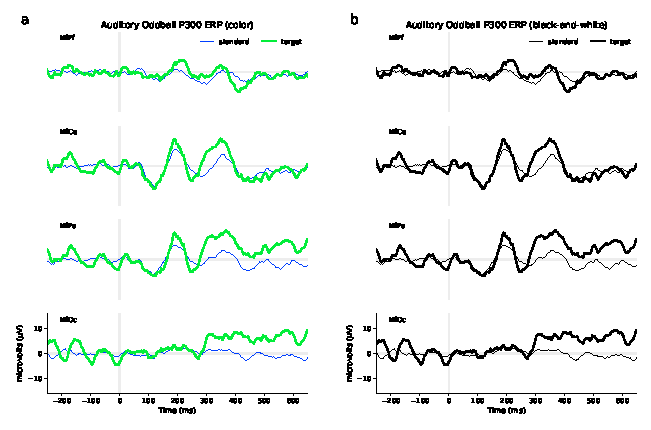
\includegraphics[width=.95\textwidth]{apa_fig1.pdf}

\end{figure}



\begin{figure}[ht]
  \caption{Reproducible figure layout and annotation. Panel a shows
    the pdf as generated by the analysis script and a stock montage
    image. Panel b shows the ``camera ready'' figure output generated
    by post-processing the generated graphic with \LaTeX{} and the
    Ti{\it k}Z drawing library as part of the documentation generation
    pipeline. The data are the same as in Figure~\zref{ms:multipanel}
  }\zlabel{ms:tikzfig} 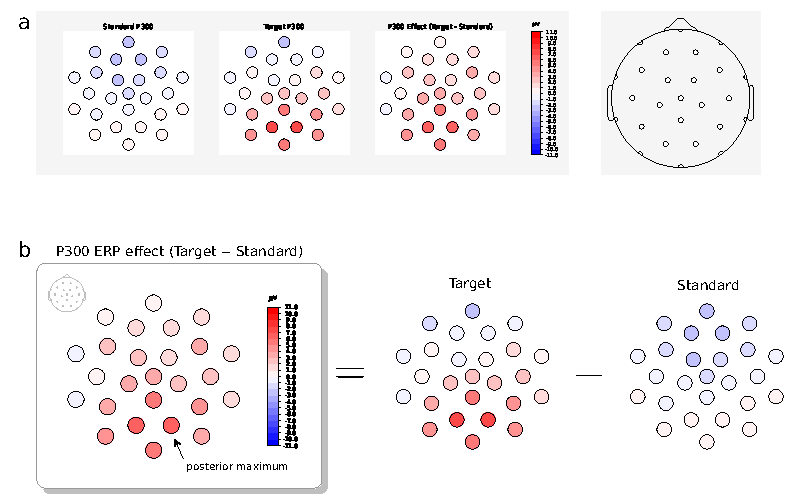
\includegraphics[width=\textwidth]{apa_fig2.pdf}
\end{figure}


%% % Figure 2
%% \begin{figure*}[ht]
%% \centering
%% \includegraphics[width=0.9\textwidth]{fig2.pdf}

%% \caption{
%%   Simple resizing and clipping can be done in LaTeX{} by tuning the
%%   options for includegraphics. This is the same .pdf plot as
%%   in Figure~\ref{fig_1} resized with to 90\% of the width of the text.
%% }\zlabel{lp_filt}
%% \end{figure*}





\subsection{Citations, masked citations, and references}

In \LaTeX{} citations in the text are indicated by typing commands
like \mintinline{latex}{\cite{}} with the author, name, year,
parenthesis information for APA style are determined when the document
is typeset. Typing the citation commands amounts to
``cite-while-you-write''. LaTeX automatically generates a bibliography
in the APA style from the corresponding .bib file (bibliography
database) according to the citations that appear in the text.  There
lots of options for citation format, see the
\mintinline{latex}{biblatex} and \mintinline{latex}{apa6} docs for
reference. For instance, the \mintinline{latex}{\parencite} command
generates a formatted citation in parentheses
\parencite{Lamport1986}. The cite command generates one without
parentheses, as in~\cite{Lamport1986}. When manuscript submission
requires citation masking for blind review, the masked variants of the
citation commands, e.g., \mintinline{latex}{\maskparencite} can be
used: \maskparencite{Lamport1986}. The masked citations are indictaed
in bold when the manuscript is typeset normally and replaced with {\it
  (1 citation removed for masked review)} when typeset with the mask
option.

The .bib file is a text file with bibliography entries that have the
usual author, title, data, publisher, fields, and a great many others,
in a specific format.  There are several options for where to get the
.bib file. Scientific literature search engines, publisher websites
routinely export citations in .bib format which can be copy-pasted
instead of tediously typed. If a reference manager is already being
used, it may also be able to export its references to .bib format. And
there are a number of reference managers that are designed from the
ground up to use .bib. As of this writing, the open-source JabRef
seems to have emerged as pick of the litter, being fully featured
enough to support general use and working across platforms. BibDesk
is another option but only runs on OSX. If other options fail, the
entry can be typed.


\subsection{Cross references}

To cross-reference between elements like tables, figures, and sections
\LaTeX{} links them via \mintinline{latex}{\label}
\mintinline{latex}{\ref} pairs. However a more general approach is to
use the \href{https://ctan.org/pkg/zref}{zref package} which links
elements with \mintinline{latex}{\zlabel} \mintinline{latex}{\zref}
pairs that work across documents which the built-in version does
not. This is particularly useful for cross-referencing information in
the Supplementary Information from the main manuscript and vice
version. When there are two or more docs and a series of figures
and/or tables and/or document sections in each and have to add or
delete another, it is mighty handy to have the references everywhere
in both documents automagically update the numbering and page
locations. Here is an example cross reference a section in the
Supporting Information, if that section title changes so does this
reference:~\ztitleref{si:analysis_nb}.  To cross-reference between
.tex documents, both documents must be compiled and this may not be
possible in all online submission systems, even those that accept .tex
format documents. For instance, the PNAS online submission system
accepts latex for manuscripts but requires .pdf for supporting
information and does not accept uploads of the auxiliary files
required by zrefs in the main manuscript which means the submission
system cannot correctly compile .tex manuscripts with zrefs.

\subsection{Tracking changes}

Revisions to a document marked and tracked in a document in the same
way as other types of formatting. With the
\mintinline{latex}{\changes} package, authors indicate the type of
change or markup, e.g., add, delete, replace, highlight, and then
bracket the relevant text, like so:
\mintinline{latex}{\added[id=TPU]{Here is some new text}}.  When the
document is type typeset in draft mode:
(\mintinline{latex}{\usepackage[draft]{changes}}), the changes are
highlighted and tagged by author. For instance \added[id=TPU]{This
  text is marked by TPU as added} and \deleted[id=ABC]{this text is
  marked by ABC as deleted}. Furthermore, \highlight[id=TPU,
  comment={is this helpful?}]{this text is marked by TPU as
  highlighted} and \replaced[id=XYZ]{this is XYZ's replacement
  text}{this text was replaced}.

In draft mode, a list of the changes can be generated by inserting the
\mintinline{latex}{\listofchanges} command, typically at the beginning
or end, though shown here at the end of this section for illustration.
Collaborators can review the changes in the pdf and add make further
revisions to the .tex document. When the document is typeset for the
final version (\mintinline{latex}{\usepackage[final]{changes}}), the
changes are applied and remaining comments, markup, and annotations
stripped, similar to accepting tracked changes in a WSYSIG
document. The draft and final versions may both be useful when
resubmission of a document following revision requires both ``clean''
version with the changes made and a draft version marked up to
indicate where the revisions were made. For cases where there are two
versions of a .tex document and the changes are not explicitly marked
up inline, the command line utility program
\mintinline{bash}{latexdiff} can be used to automatically generate a
single pdf with the differences between the versions indicated as in
changes. Both of these features are best suited to marking revisions
and changes in the text of relative similar documents and are not
well-suited to track massive restructuring or revisions to figures and
tables. Here is the list of changes explicitly marked up in the
previous paragraph.

\listofchanges


\subsection{Compositing documents: files and file formats}

Various files and formats are required go submit and publish a
research report. These may include a main editable manuscript
(document), supporting information (document, data), figures (vector
and raster image graphics files), tables, and bibilographic
info. Journals and publishers have divergent interests (readability
for evaulation in review vs. production for print and digitial
formats) and (thus) different requirements for document
preparation. This is further complicated by open-access policies that
require authors to deposit a final pre-publication manuscript if the
publisher won't (but most do, eventually).  For submission to
Psychological Science for instance, the file formats are \LaTeX (.tex)
for editable text and Portable Document Format (.pdf) for graphics, a
vector format that is scalable without loss of resolution. To submit
the report to the journal for review the .tex and .pdf graphic files
composited into a single .pdf file and all files
uploaded~\cite{PsychSciSubmissions2020, PsychSciFigs2013}. Whereas the
journal submission portal requires the a single composited document
with text and graphics all in one, the publisher's portal requires the
separate editable text and graphics files, i.e., the .tex and graphics
.pdfs.

Working with \LaTeX{} simplifies some aspects of this by allowing
files in different digital formats to be included in documents in
various ways. As illustrated by linking results and abitrary text for
narrative descriptions and tables, separate files of \LaTeX{} can be
inserted directly into the document as if typed in place. This allows
the tables to be reproducibly prepared as separate files (as required
by some publishers) and also incorporated in exactly the same form in
the body of the manuscript (as also required by these publishers). The
same holds for the camera ready graphics for Figure~\zref{ms:multipanel} and
\zref{ms:tikzfig} which are also separate files included as-is in the
mansucript. Additionally the \mintinline{latex}{\includepdf} package,
allows all or selected pages of a multi-page PDF documents to be
included in a \LaTeX{} as demonstrated in by the Supplementary
Informatinon that includes the entire PDF of the fully executed data
analysis Jupyter Notebook.  Finally, the \mintinline{latex}{\minted}
package used extensively throughout this document will import the
contents of separte files into the \LaTeX{} document and also
highlight the code according to the syntax of the specfic language,
e.g., Python, R, \LaTeX{} which is of great value in documenting
scripted reproducible research pipelines. The Supplemental Information
demonstrates this by importing and highlighting all the \LaTeX{} files
used in the producition and reproduction of this tutorial report.

\subsection{Author manuscripts}

Whereas journals may require submission as a double spaced manuscript,
the published articles typeset single space in two columns with
figures and tables where they belong are generally easier to read.
Switching the \mintinline{latex}{documentclass} option from man
(manuscript) to jou (journal) typesets the document in a
more-nearly-journal-like format (Figure~\zref{ms:apa67_jou}), which
may be useful for distributing working drafts or post-publication
author manuscripts during a publisher's embargo period.

\begin{figure}
\caption{Example of typesetting this document with the jou option}
\zlabel{ms:apa67_jou}
\centering
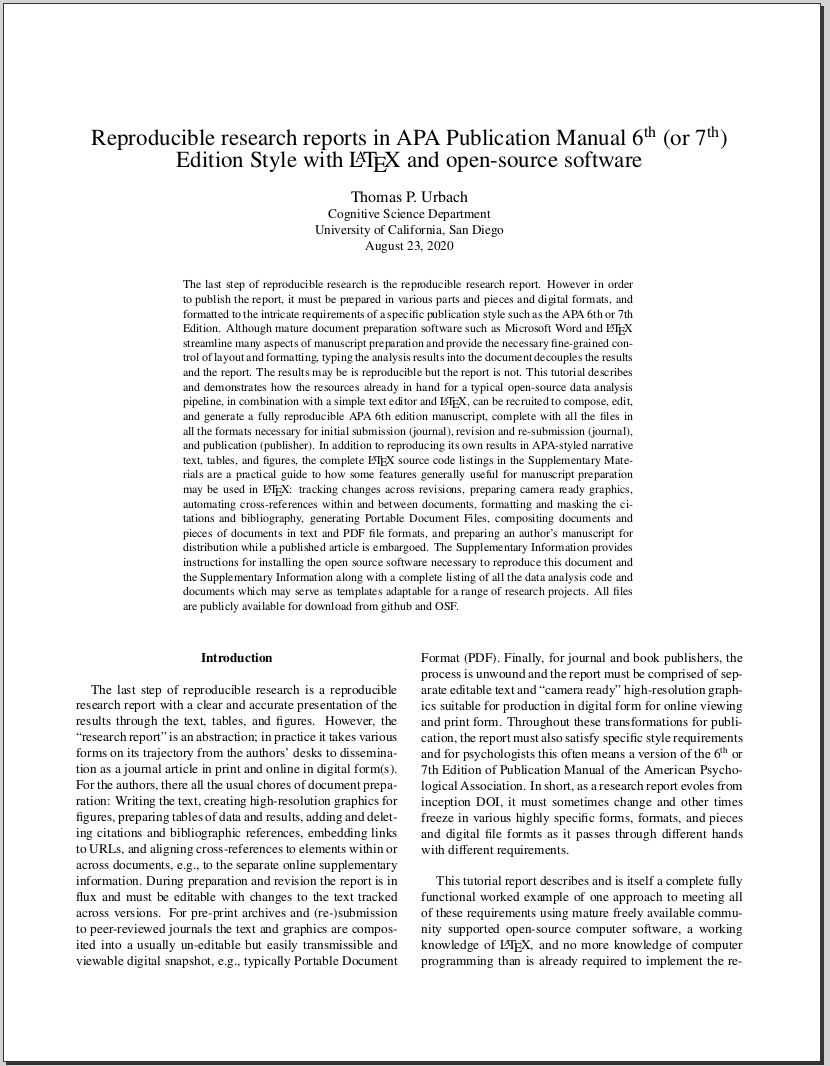
\includegraphics[width=.65\textwidth]{images/apa67_jou.png}
\end{figure}


\section{Conclusion}

There are many ways to prepare a research report but far fewer to do
 so reproducibly while at the same time satisfying the requirements of
publication styles and online journal submission and production
platforms.  This report illustrates one approach that does so and
dovetails with best practices in open science data analysis. Once
a reproducible analysis in place, the additional cost of the
reproducible report is acquiring a working knowledge of \LaTeX{} and
if necessary Ti{\it}Z.

\newpage
\printbibliography

\end{document}

